When analyzing diffraction data using this program,
not all of the pixels in an image have to be used in
the data analysis. In order to make the program
ignore certain pixels when doing the analysis, this
program allows for two types of pixel masking:
threshold masking and polygon masking. You can apply
a mask to a diffraction image by going to the
\gui{Masking} tab of the GUI. There is a screen
shot in figure~\ref{masking_page} of this tab.

\section{Threshold Masking}

\begin{SCfigure}[1][htb]
    \centering
    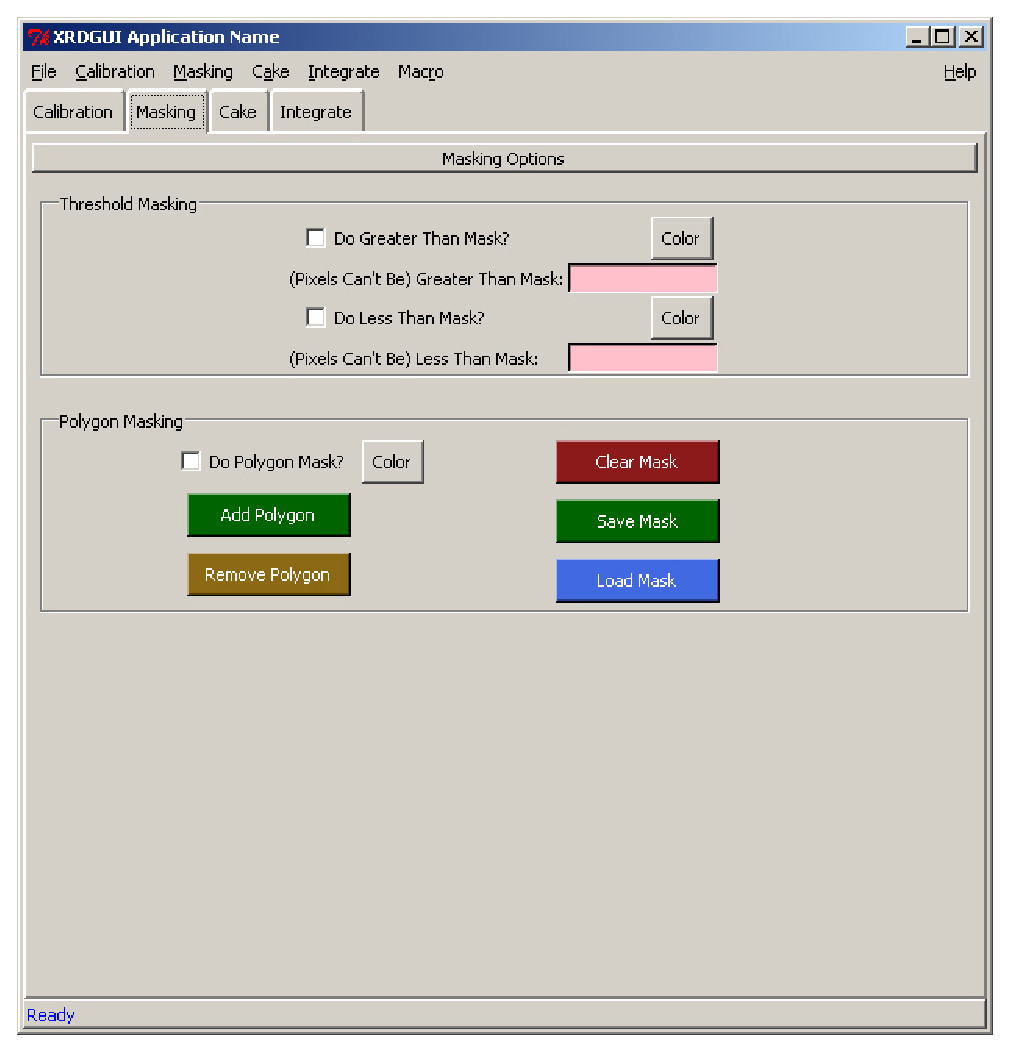
\includegraphics[scale=.75]{figures/masking_page.eps}
    \caption{A screen shot of the pixel masking tab. This
    tab allows for threshold masking and polygon masking. 
    Threshold masking can be used to have the program 
    ignore all pixels with intensity above or below
    a certain value when doing data analysis. 
    Polygon masking can be used to have the programme
    ignore all pixels in certain areas of the image
    when doing data analysis.} 
    \label{masking_page}
\end{SCfigure}

The top half of the \gui{Masking} tab is devoted to 
threshold masking. Threshold masking allows all pixels, 
either above a certain intensity value or below a certain 
intensity value, to be ignored when doing diffraction 
analysis. If you want to apply a mask that will cause 
all pixels greater than a certain value to be ignored,
you can select the \gui{Do Greater Than Mask?} option.
The \gui{(Pixel's Can't Be) Greater Than Mask} input 
lets you specify what the maximum pixel should be.
Correspondingly, the \gui{Do Less Than Mask} check box
allows you to require that the program ignores all
pixels below a certain value when doing diffraction
analysis. The lowest value can be specified by the 
\gui{Less Than Mask} input. 

\begin{SCfigure}[1][htb]
    \centering
    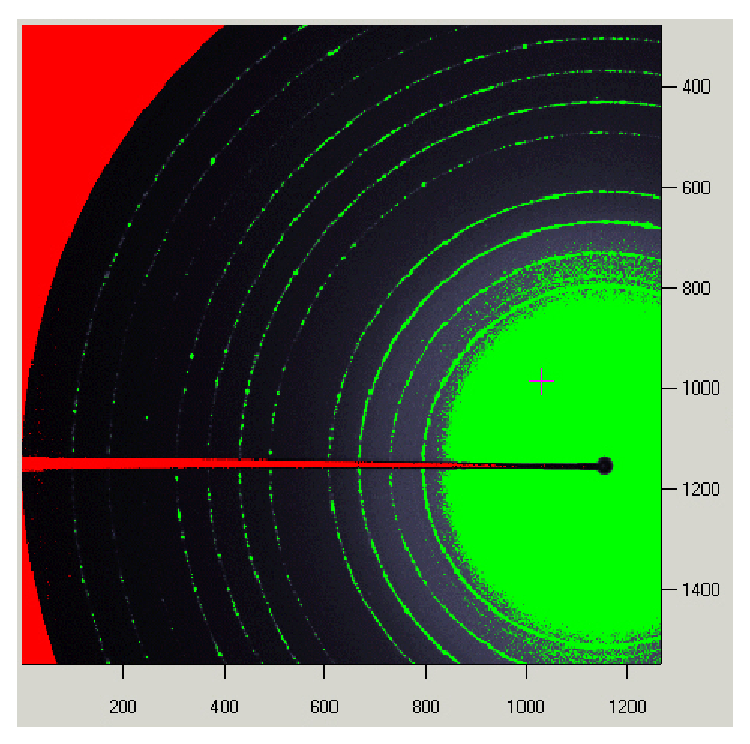
\includegraphics[scale=.75]{figures/Threshold_Masking.eps}
    \caption{Here is an example of diffraction with a
    greater than mask and less than mask applied.
    All pixels in this image with intensity greater than 5000 
    have been colored green. All pixels in this image with 
    intensity less than 30 have been colored red. Applying
    an intensity mask can be a useful way to see if a detector's
    pixels have been overloaded and it can also be used to
    ensure that no overloaded pixels are used in subsequent
    data analysis.}
    \label{Threshold_Masking}
\end{SCfigure}

When you apply a threshold mask, the pixels over this threshold 
will be colored differently on the diffraction and cake image. 
You can specify what color you want these masked pixels to show 
up as by with the \gui{Color} selector button next to the greater 
than and less then masks. Figure~\ref{Threshold_Masking} shows 
what the diffraction image looks like when all the pixels with 
intensity above 5000 were masked 
and colored green and all pixels below 30 were masked and
colored red.

If you apply a greater than mask and then save the cake data
to a file, any of the pixels that are larger than the greater
than mask are outputted with value -2. If you apply a less 
than mask and then save the cake data, any of the pixels
that are smaller than the less than mask are saved as -3.
If you need to analyze caked data further on, you need to
make sure to account for this. When you apply a threshold
mask and then perform an intensity integration, any of the 
too high or too low pixels are simply ignored when calculating
average intensity. 

\section{Polygon Masking}

\begin{SCfigure}[1][htb]
    \centering
    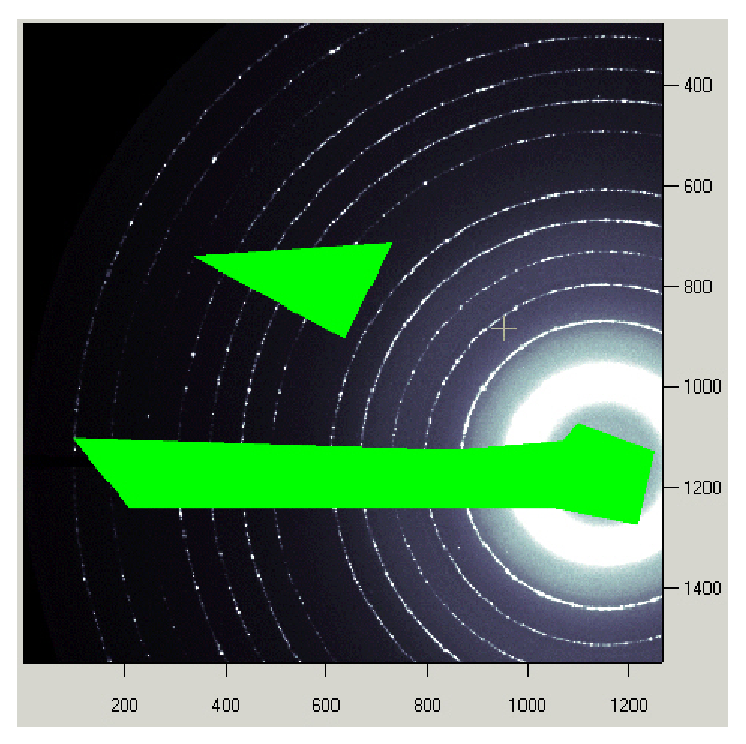
\includegraphics[scale=.75]{figures/Displayed_Polygon.eps}
    \caption{In this screen shot of a diffraction image, we
    see two polygon masks that have been added to the
    image. One of them is blocking the beam stop and
    the other is just there for show. Note that this program 
    can use multiple polygons.}
    \label{Displayed_Polygon}
\end{SCfigure}

Sometimes, large areas of a diffraction image are bad 
and should not be used in any data analysis. For example, 
often a beam stop blocks part of the diffraction data 
and the pixels which were blocked by the beam stop 
should be ignored. Also, sometimes parts of the experimental 
setup can block parts of the detector and those areas 
of the data must be ignored. This is called shadowing.
To allow for this sort of masking, the program has a 
polygon masking feature. You can draw polygons around 
certain parts of the diffraction image and those parts 
of the image will not be used in any diffraction analysis. 
The program can handle as many separate polygons as you 
want to use.

Once polygons have been added to the image (as is 
described below), you can have these polygons
used when performing data analysis by checking the
\gui{Do Polygon Mask?} check box. Once you do that,
these polygons will be displayed on the diffraction
and cake image. This is to say that any pixel in
the diffraction or cake image that is inside of one of
the polygons will be displayed with a different color.
An example of polygons on a diffraction image are 
shown in figure~\ref{Displayed_Polygon}.

You can change this color using the \gui{Color} button
next to the \gui{Do Polygon Mask?} check box.
When you save out cake data, any pixels inside of 
a polygon mask will be given an intensity 
value of -4. When you perform an intensity integration,
any of the masked pixels will simply be ignored when
calculating average intensities.

\begin{SCfigure}[1][htb]
    \centering
    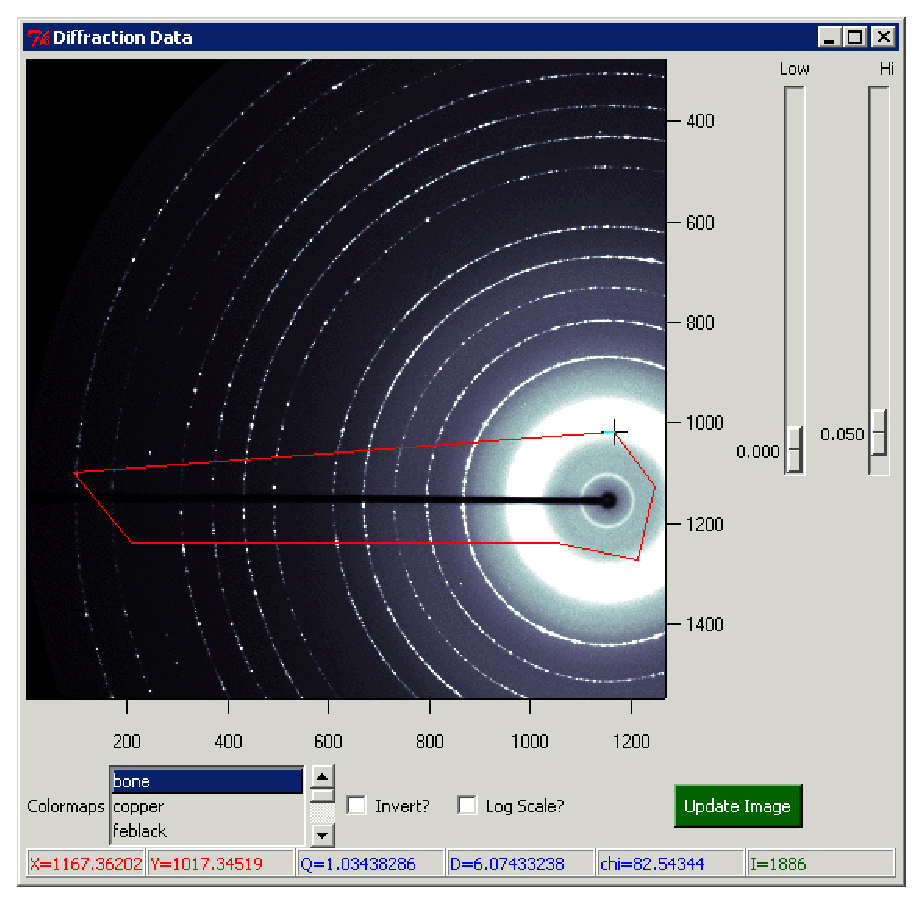
\includegraphics[scale=.75]{figures/Adding_Polygon.eps}
    \caption{Here is a screen shot of the diffraction
    image where the user is adding a new polygon 
    mask that will be added into the program.
    This mask will completely cover up the beam stop
    and ensure that those values are not later used
    when performing an intensity integration.}
    \label{Adding_Polygon}
\end{SCfigure}

To add a polygon mask to the image, you have to push
the \gui{Add Polygon} button. When you push it, this
button will stay stuck. So pushing it enters you into
polygon drawing mode. When you are in this mode, 
the diffraction image will behave differently. You will not
be able to do any zooming or panning on the image. Instead,
when you left click on the diffraction image, you will 
begin drawing the polygon. The first left click on the
image will add the 
first vertex of the polygon. Each success left click
will add another vertex to the polygon. When you want to
finish drawing the polygon (by adding one final vertex to
it), you right click where you want that final polygon to
be. Once you right click, the program will exit the 
\gui{Add Polygon} mode and the regular zooming features of
the diffraction image will take over.
That polygon will then be added to the program. 
You can add as many polygons to the 
program as you wish. An example of drawing a 
polygon is shown in figure~\ref{Adding_Polygon}.
If you are are part way through drawing a polygon 
and decide that you don't like it any more, you can
simply unpush the \gui{Add Polygon} button and the
polygon in progress will be removed and the regular
bindings will take over.

\begin{SCfigure}[1][htb]
    \centering
    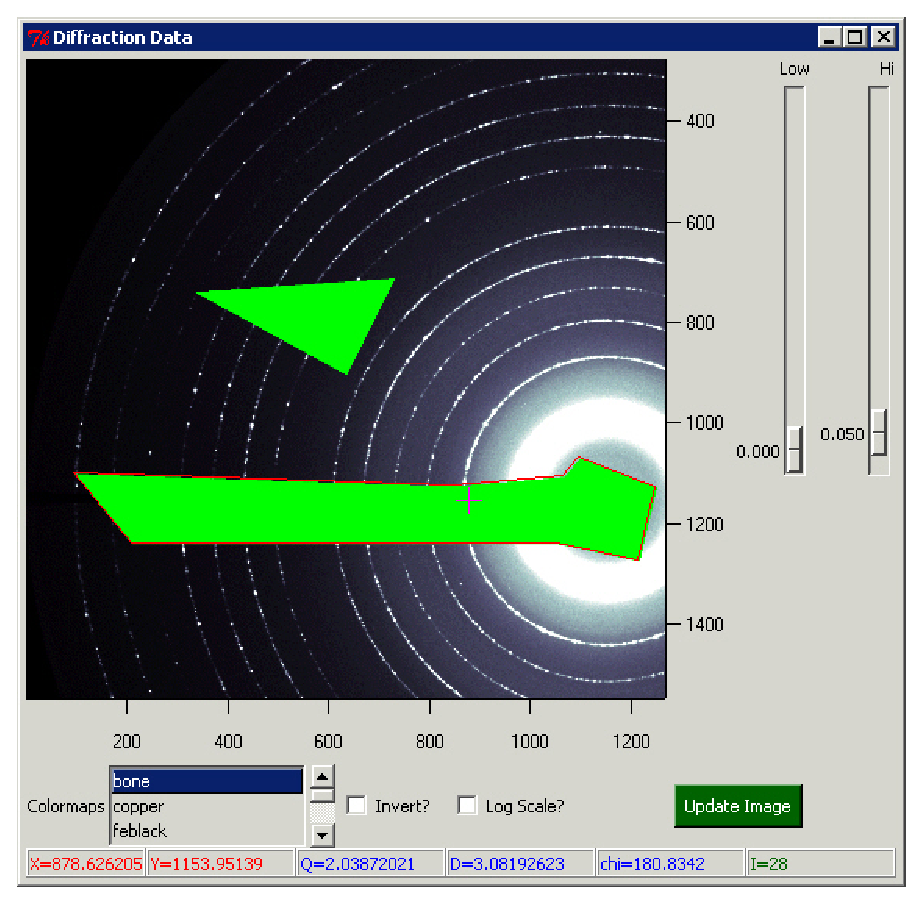
\includegraphics[scale=.75]{figures/Removing_Polygon.eps}
    \caption{Here is a screen shot of the diffraction
    image where the user is in the process of removing
    a polygon. To remove a polygon, you have to push the
    \gui{Remove Polygon} button and then click on the
    polygon in the diffraction image that you want to
    remove. When you mouse over a polygon,
    the program will display a border around it so that
    you know that that particular polygon is the one
    that will be deleted.}
    \label{Removing_Polygon}
\end{SCfigure}

If you want to remove a polygon that is already in
the program, you can push the \gui{Remove Polygon}
button. Like the \gui{Add Polygon} button, this
button will stay pushed and change the bindings of 
the diffraction image. When you now click on the
diffraction image while the mouse is on top of a
polygon, that polygon will be removed from the file.
After deleting a polygon, the program will leave
the \gui{Remove Polygon} mode and diffraction 
image will regain the regular zoom features.
An example of removing a polygon is shown
in figure~\ref{Removing_Polygon}
If you have a change of heart after pushing the
\gui{Remove Polygon} button and no longer want to
remove a polygon, you can simply unpush the button
and the program will leave the \gui{Remove Polygon}
mode. A gotcha that can easily happen when you are
using the diffraction image is that you push the
\gui{Add Polygon} or \gui{Remove Polygon} button
and then forget that you pushed it. If you do so,
the diffraction image will start behaving as
previously described. Don't forget that you can 
always unpush the button to return the program to
its normal state.

If you want to remove all the polygons in one go,
you can use the \gui{Clear Mask} button. If you
want to save all the polygons inside of the 
program to a file, you can use the \gui{Save Mask}
button. If you want to load all of the polygons
from a file into the program, you can use the
\gui{Load Mask} button. The file format for polygon
mask files is very simple. For example, saving
out the polygons shown in figure~\ref{Displayed_Polygon}
creates the file:
\begin{lstlisting}[caption={'A demonstrative polygon mask file'}]
# Polygon(s) drawn on Thu Feb 07 00:00:21 2008
93.140587183	1098.06704199
208.013978042	1237.77792276
1052.48863517	1237.77792276
1213.93231962	1271.92947139
1248.08386825	1126.00921814
1095.95424252	1067.02017959
1064.90738013	1104.27641447
847.579343365	1122.9045319

332.201427619	737.923438212
633.355992844	902.471808902
729.601266267	709.981262058
\end{lstlisting}
The format for these files is to have each line have
an ($x$,$y$) coordinate for one of the nodes in
the polygon. Multiple polygons are separated by
newlines and there should be no other formatting.
Note that as in figure~\ref{Displayed_Polygon},
one of the polygons has only three vertices
and is a triangle while the other has many
vertices and is a more complicated shape.
As always, comment lines beginning with \# are 
ignored except when they are between coordinates
in which case they also signify the division of
separate polygons.

Masking Caked Plots


\section{Masking Caked Plots}

\begin{figure}[htb]
    \centering
    \subfloat[A rectangular polygon mask in 
    the middle of a diffraction image]{
    \label{box_mask_diffraction}
    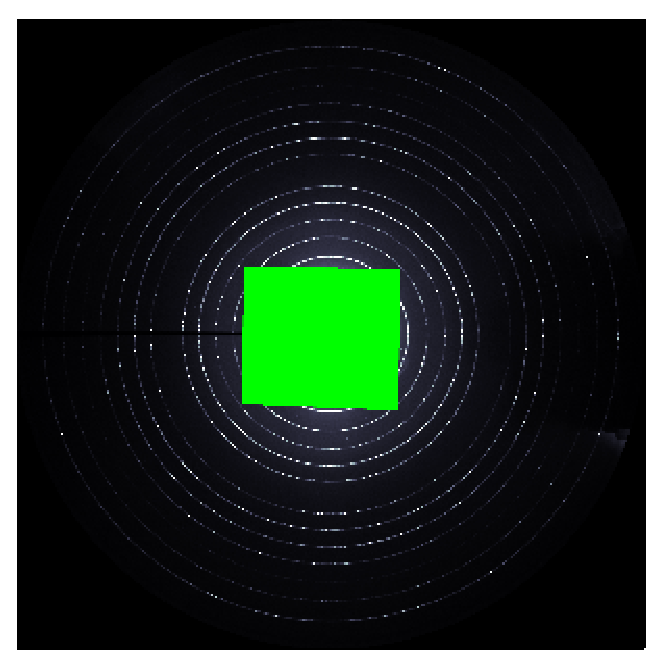
\includegraphics[scale=.75]{figures/box_mask_diffraction_image.eps}}
    \subfloat[The same rectangular mask as 
    seen on the caked plot]{
    \label{box_mask_cake}
    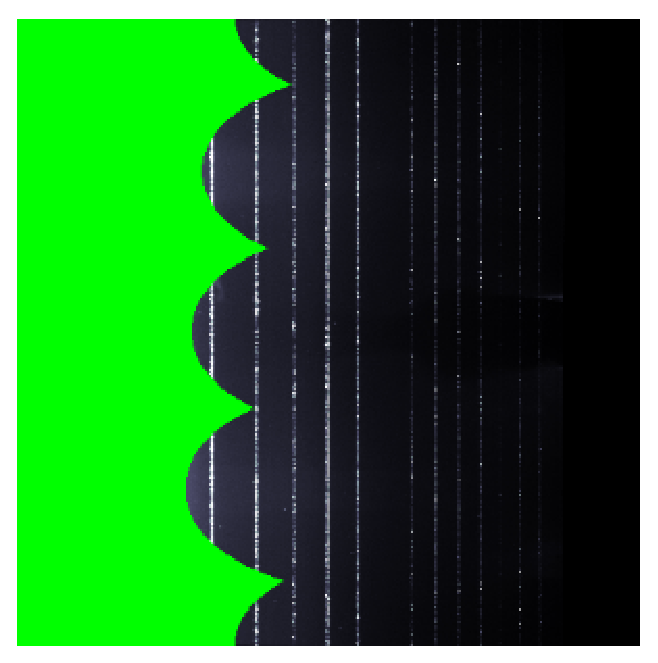
\includegraphics[scale=.75]{figures/box_mask_cake_image.eps}}
    \caption{An example of how a relatively simple
    shape drawn on a diffraction image can show
    up as a very complicated shape on a caked
    plot. (a) is a diffraction image with a square 
    mask and (b) is a cake of the same image with 
    the same mask.}
    \label{box_mask}
\end{figure}

Any polygon mask or threshold mask will also show 
up on the caked plot whenever it should be shown
on the diffraction image. Polygon can be distorted
into much different shapes on the caked plot. 
Figure~\ref{box_mask} shows an example of this.



